%
% tangente.tex -- Tangente an eine Kurve
%
% (c) 2017 Prof Dr Andreas Müller, Hochschule Rapperswil
%
\documentclass[tikz]{standalone}
\usepackage{times}
\usepackage{txfonts}
\usepackage{pgfplots}
\usepackage{csvsimple}
\usetikzlibrary{arrows,intersections}
\begin{document}
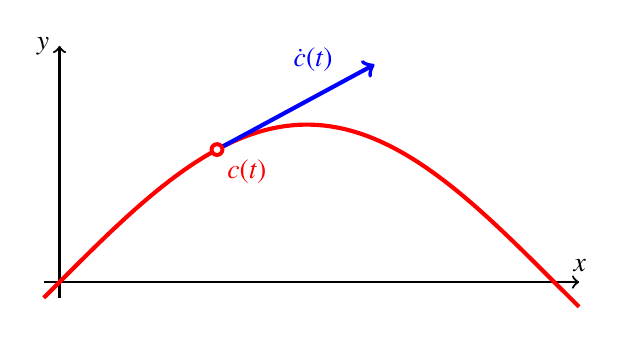
\begin{tikzpicture}[thick,scale=2]
\coordinate (O) at (0,0);

\draw[->] (-0.1,0)--(3.3,0) coordinate[label={above:$x$}];
\draw[->] (0,-0.1)--(0,1.5) coordinate[label={left:$y$}];

\draw[red,domain=-0.1:3.3,line width=1.5,samples=100] plot (\x,{sin(180 * \x/3.14159)});

\draw[->,blue,line width=1.5]
(1,{sin(180 * 1 / 3.14159)})--(2,{sin(180 * 1 / 3.14159)+cos(180 * 1 / 3.14159)});

\draw[red,fill=red] (1,{sin(180 * 1 / 3.14159)}) circle[radius=0.04] {};
\draw[red,fill=white] (1,{sin(180 * 1 / 3.14159)}) circle[radius=0.03] {};

\node at (1,{sin(180 * 1 / 3.14159)}) [below right,red] {$c(t)$};
\node at (1+0.8,{sin(180 * 1 / 3.14159)+0.8*cos(180 * 1 / 3.14159)}) [above left,blue] {$\dot c(t)$};

\end{tikzpicture}
\end{document}


